\documentclass[../../main.tex]{subfiles}

\begin{document}

\section{Introduction}

Steganography is the technique of hiding a message inside another message or a
physical object.\cite{steganography-definition}
The word \emph{steganography} comes from the Greek word
\emph{steganographia}, which is the combination of \emph{steganós} meaning
``covered'' and \emph{-graphia} meaning ``writing''.

The first testimonials of the use of steganography date back to 440 BC in Greece
mentioned by Herodotus in his \emph{Histories} where he tells the story of Histitateus who tattooed a message on the shaved head of a servant of his
and after the hair had regrown, he sent him to Aristagoras.
Other historical exaples come from the story of Jeremiah Denton, who fell prisoner in 1966 during the korean
war and encoded an help message in his blinking rhythm which transmitted during a TV report and from microdots
embedded in paper or in clothes used by espionage agents during and after the
World War II.

With the advent of the \emph{Digital Era} steganography has found fertile ground. Nowdays information can easily
be concealed in almost every type of file in ways which are basically invisible to the common user. Images, videos and documents 
can contain hidden text as well as malicious code embedded into them, representing a serious threat for cybersecurity. 
Sometimes the message could also be encrypted to be unreadable even for active searchers. Although this is the domain of cryptoanalysis. 

In this paper we will focus on steganalysis, the study of detecting and, if
possible, recovering hidden messages encoded using steganography. The ways in
which it can be performed, examples of its application in known cases and
the cybersecurity implications of its use in digital communication systems.

The Field on Information Security Systems is indeed vast and will require much
more space than the one we have. Here we attach a map which describes shortly
the structure.

\begin{figure}[h]
    \centering
    \caption{Map of Information Security Systems \cite{modern-text-hiding}}
    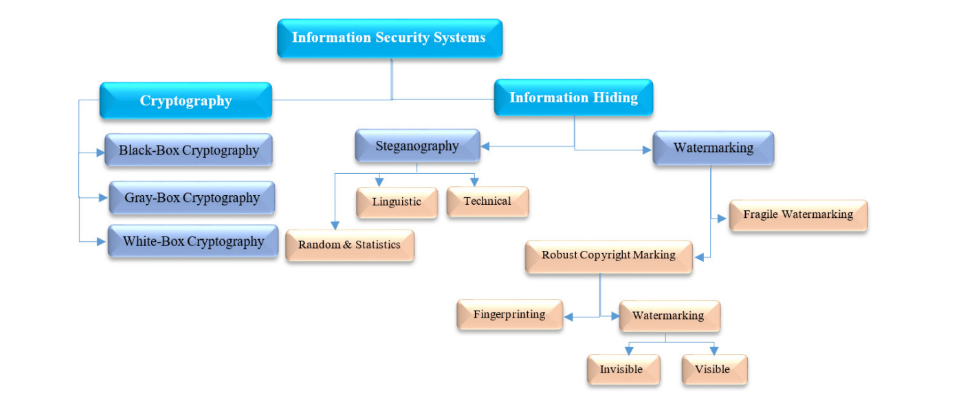
\includegraphics[scale=0.65]{map.png}
\end{figure}

\end{document}